We implemented a chat using NodeJs and the node-serialport library.
The chat has a command line interface and offers the following functionalities:
- configure used device
- configure retrans, difs, cwmin and cwmax with command line parameters
- logging to a .csv file
- fallback to default values if nothing provided
- broadcast and private messages
- "spam" mode to generate saturation traffic
Screenshots:
\begin{figure}[htp]
\centering
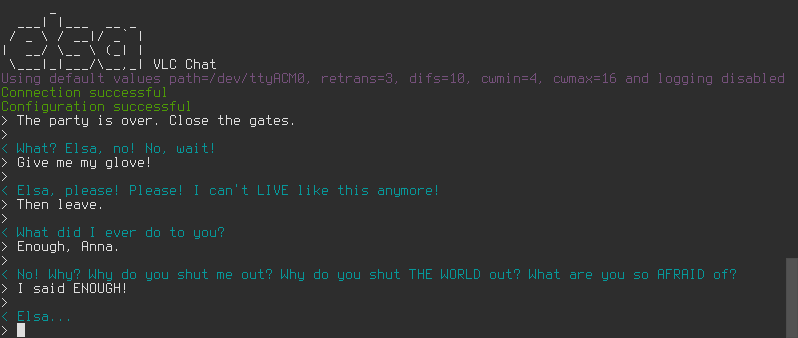
\includegraphics[scale=0.4]{../img/elsa_1.png}
\caption{}
\label{}
\end{figure}
\begin{figure}[htp]
\centering
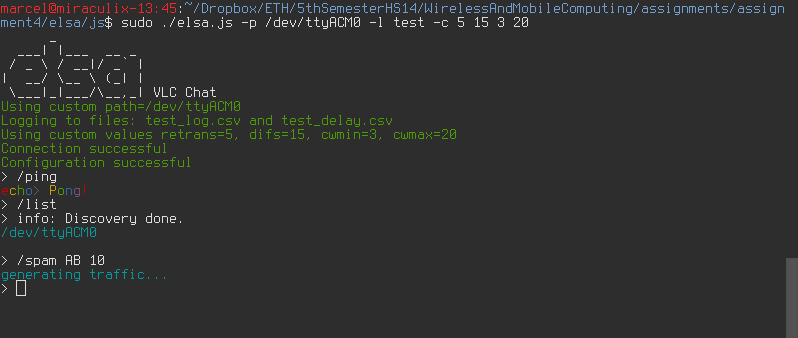
\includegraphics[scale=0.4]{../img/elsa_2.png}
\caption{}
\label{}
\end{figure}
\begin{figure}[htp]
\centering
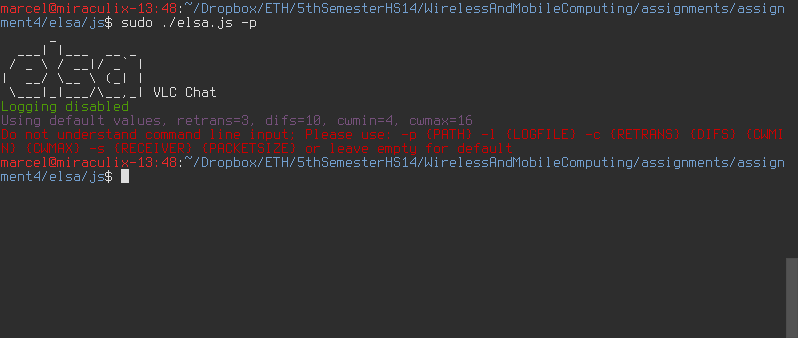
\includegraphics[scale=0.4]{../img/elsa_3.png}
\caption{}
\label{}
\end{figure}

Code see attached zip file code.zip.